% --------------------------------------------------------------
% This is all preamble stuff that you don't have to worry about.
% Head down to where it says "Start here"
% --------------------------------------------------------------

\documentclass[12pt]{article}

\usepackage[margin=1in]{geometry}
\usepackage{amsmath,amsthm,amssymb}
\usepackage{graphicx} %This allows to include eps figures
\usepackage{subcaption}
\usepackage[section]{placeins}
\usepackage{layout}
\usepackage{etoolbox}
\usepackage{mathabx}
\usepackage{animate}
\usepackage{array}
% This is to include code
\usepackage{listings}
\usepackage{xcolor}
\definecolor{dkgreen}{rgb}{0,0.6,0}
\definecolor{gray}{rgb}{0.5,0.5,0.5}
\definecolor{mauve}{rgb}{0.58,0,0.82}
\lstdefinestyle{Python}{
    language        = Python,
    basicstyle      = \ttfamily,
    keywordstyle    = \color{blue},
    keywordstyle    = [2] \color{teal}, % just to check that it works
    stringstyle     = \color{green},
    commentstyle    = \color{red}\ttfamily
}

\newenvironment{conditions}
  {\par\vspace{\abovedisplayskip}\noindent\begin{tabular}{>{$}l<{$} @{${}={}$} l}}
  {\end{tabular}\par\vspace{\belowdisplayskip}}

\newcommand{\N}{\mathbb{N}}
\newcommand{\Z}{\mathbb{Z}}

\newenvironment{theorem}[2][Theorem]{\begin{trivlist}
\item[\hskip \labelsep {\bfseries #1}\hskip \labelsep {\bfseries #2.}]}{\end{trivlist}}
\newenvironment{lemma}[2][Lemma]{\begin{trivlist}
\item[\hskip \labelsep {\bfseries #1}\hskip \labelsep {\bfseries #2.}]}{\end{trivlist}}
\newenvironment{exercise}[2][Exercise]{\begin{trivlist}
\item[\hskip \labelsep {\bfseries #1}\hskip \labelsep {\bfseries #2.}]}{\end{trivlist}}
\newenvironment{reflection}[2][Reflection]{\begin{trivlist}
\item[\hskip \labelsep {\bfseries #1}\hskip \labelsep {\bfseries #2.}]}{\end{trivlist}}
\newenvironment{proposition}[2][Proposition]{\begin{trivlist}
\item[\hskip \labelsep {\bfseries #1}\hskip \labelsep {\bfseries #2.}]}{\end{trivlist}}
\newenvironment{corollary}[2][Corollary]{\begin{trivlist}
\item[\hskip \labelsep {\bfseries #1}\hskip \labelsep {\bfseries #2.}]}{\end{trivlist}}



\begin{document}

% --------------------------------------------------------------
%                         Start here
% --------------------------------------------------------------

%\renewcommand{\qedsymbol}{\filledbox}

\title{Assignment 7}%replace X with the appropriate number
\author{Nalet Meinen and Pascal Wyss\\ %replace with your name
Finite Element Analysis I
}
\maketitle

\begin{figure}[!htb]
  \centering
  \vspace*{1cm}
  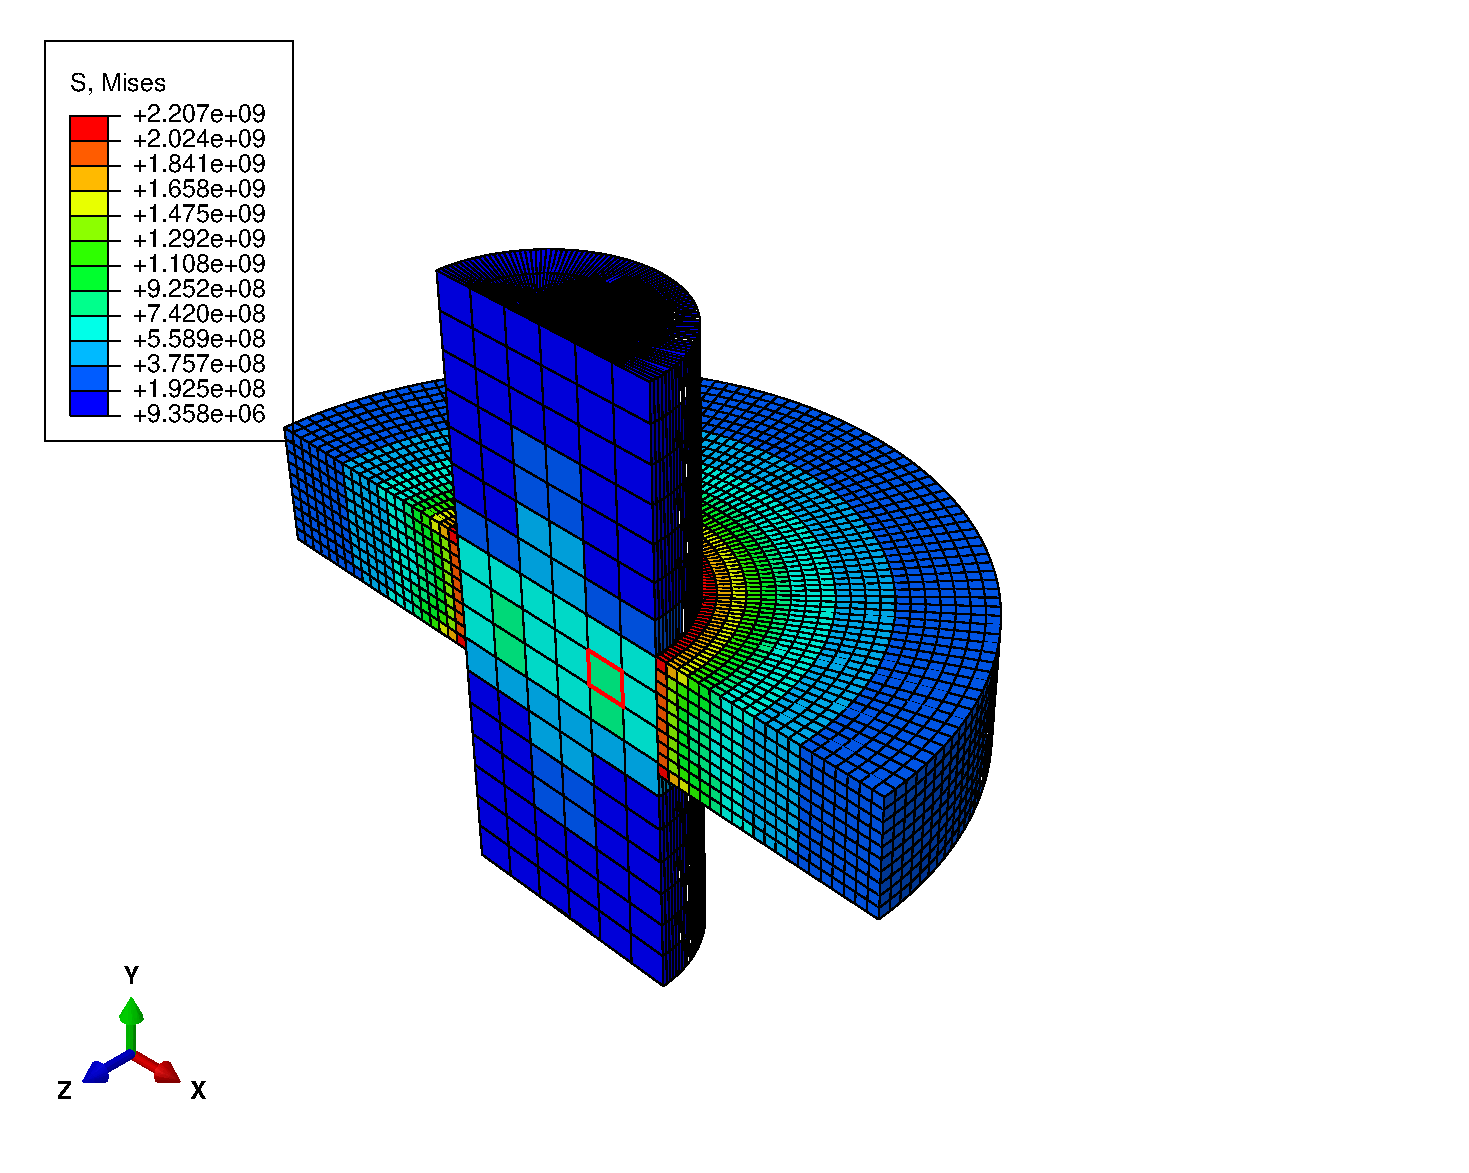
\includegraphics[trim={1cm 2cm 2cm 2cm},clip,width=1.0\linewidth]{pics/stress3d}
  \label{fig:0}
\end{figure}

\newpage

\section*{Abstract}
In this assignment we investigate the a cooling disc which is mounted on a shaft.
The occuring stresses after cooling are then assessed.

\tableofcontents
\pagebreak
\section{Introduction}

The disc is heated up to increase its diameter, then cooled down to form an interference fit.
This is a common procedure in mechanics to fit parts together (e.g. bearings on shafts).
It is therefore interesting to know, by how much the disc has to be heated in order to
get an inside diameter which fits over the shaft. In a practical application, this could be used
to specify manufactoring tolerances.



\noindent As shown in Figure \ref{fig:1}, the fibers are orientated differently in both simulations.

\newpage
\section{Methods}

\subsection{Modelling}

It is important to sequence the model into different steps. Contacts are only activated after both
instances are clear of each other (after heating up the disc). 

\subsection{Holzapfel-Gasser-Ogden Framework}

We use the Holzapfel-Gasser-Ogden approach to model the biomechanical behaviour of our
sample. This approach targets the anisotropic behaviour of the material with multiple
layers of fibers at different angles. This is required in order to achieve a relatively
realistic distribution of forces and strains within the sample.\cite{holzapfel}




\pagebreak
\section{Results and Discussion}

The results vary greatly with different mesh sizes. Especially when using quilt plots,
results may differ quite heavily from one mesh to another, as there is no averaging between elements.
Quilt plots are good for evaluation on an element-by-element basis.


\begin{figure}[!htb]
  \centering
  \begin{subfigure}{.5\textwidth}
    \centering
    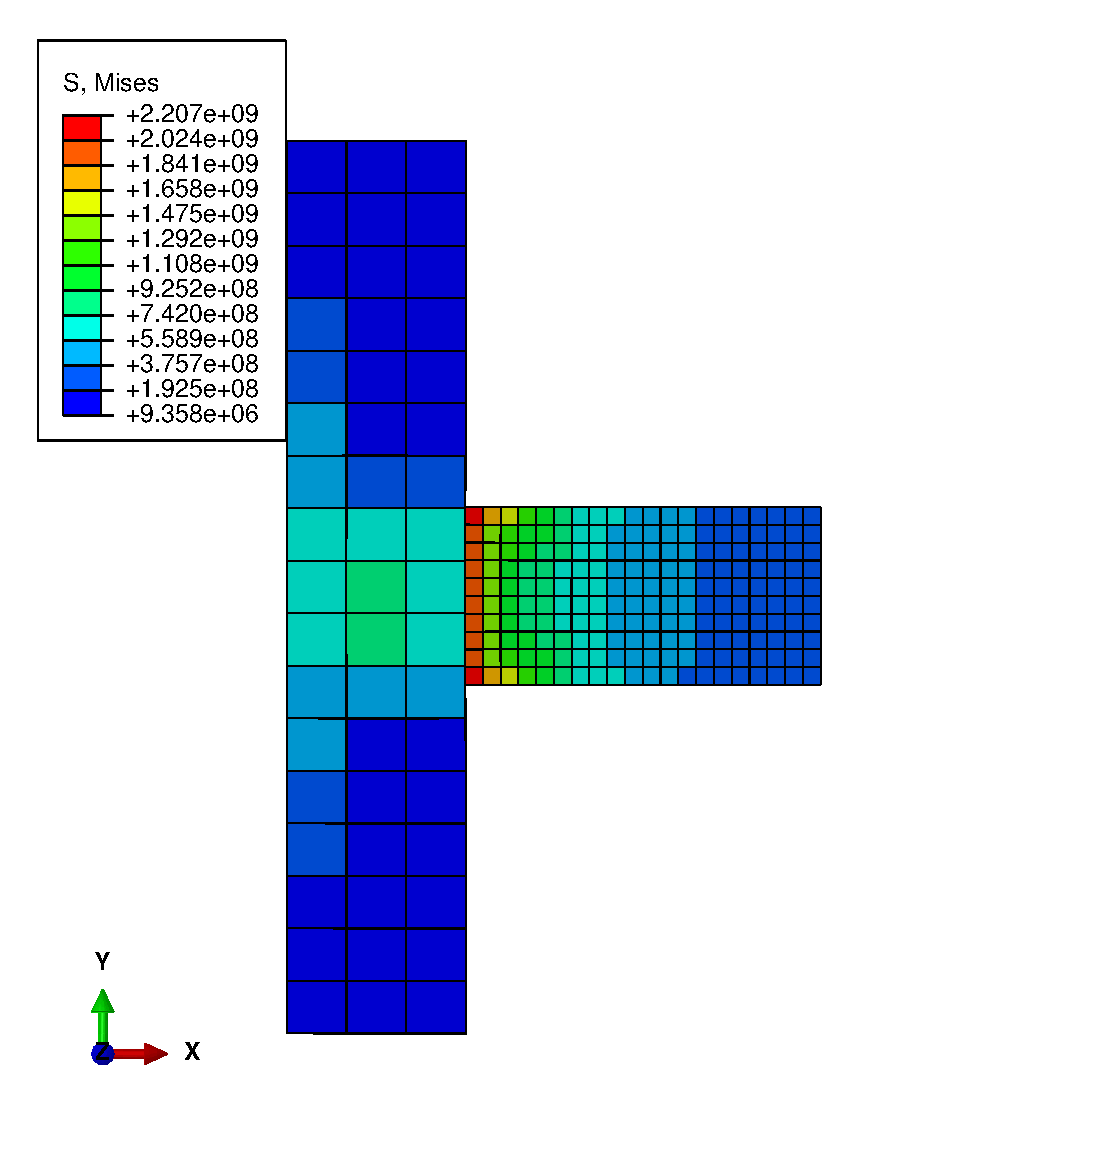
\includegraphics[width=0.95\linewidth]{pics/stress}
    \caption{Stresses with }
  \end{subfigure}%
  \begin{subfigure}{.5\textwidth}
    \centering
    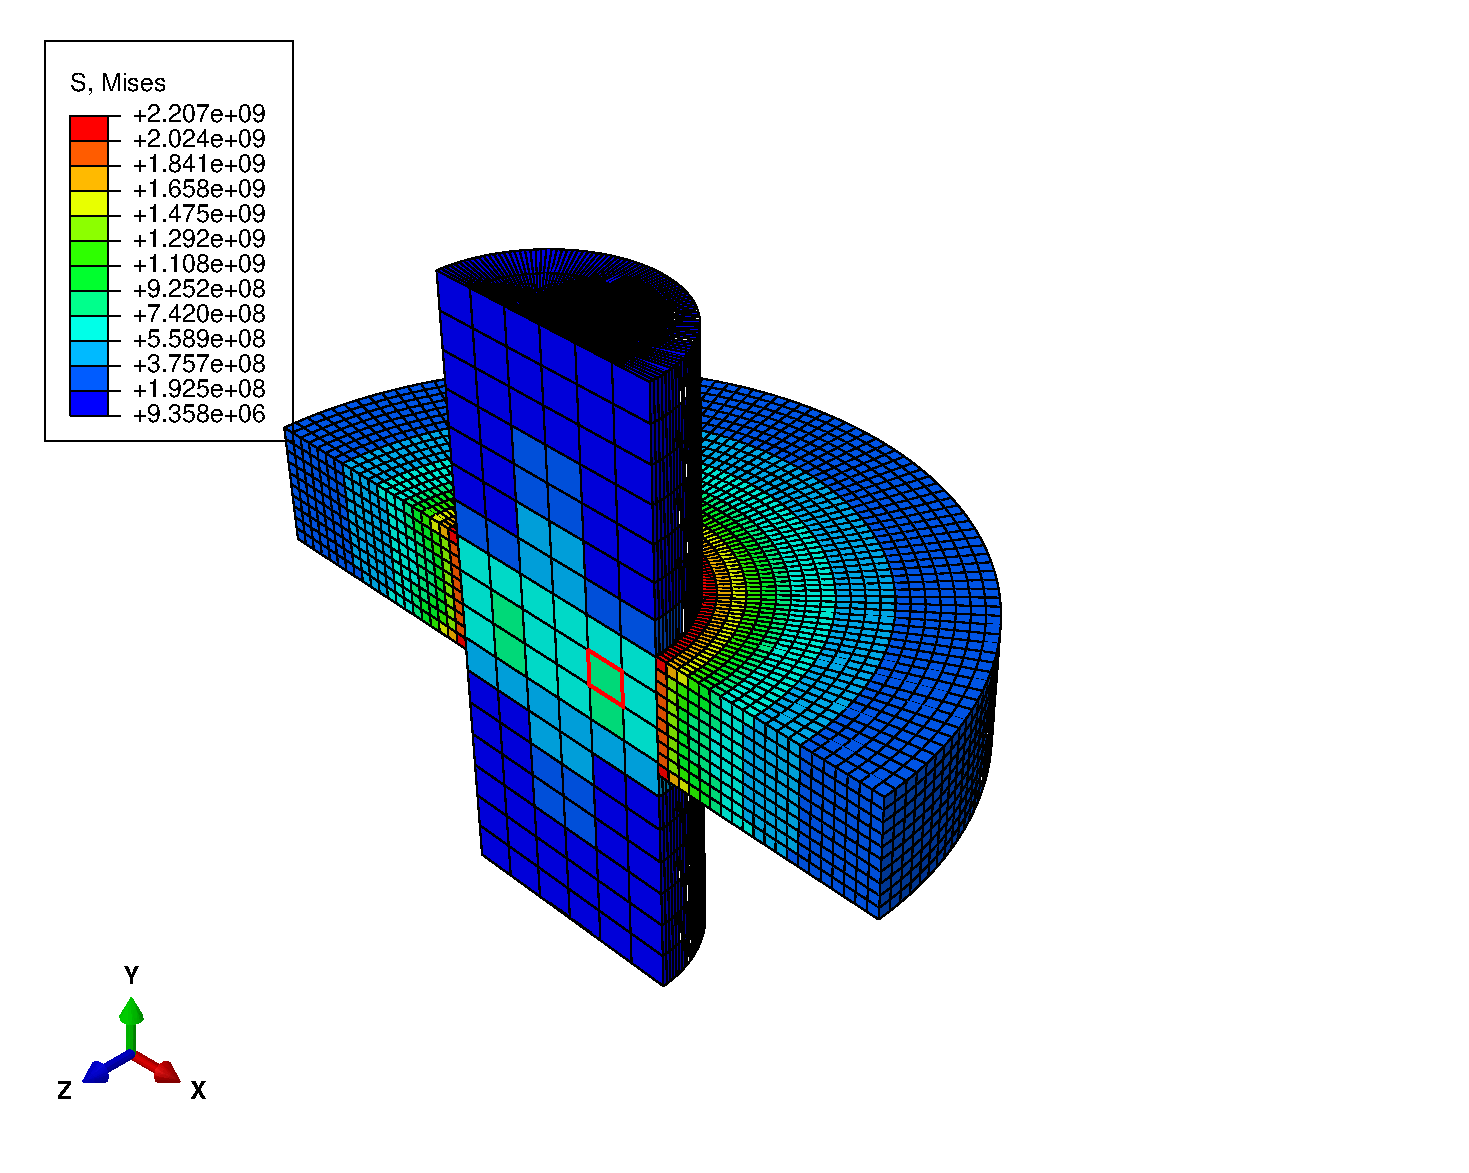
\includegraphics[width=0.95\linewidth]{pics/stress3d}
    \caption{Stresses with }
   \end{subfigure}
  \caption{Stresses on Sample}
  \label{fig:4}
\end{figure}

\pagebreak
\subsection(conclution)


\pagebreak
\begin{thebibliography}{9}
\bibitem{latexcompanion} 
Michel Goossens, Frank Mittelbach, and Alexander Samarin. 
\textit{The \LaTeX\ Companion}. 
Addison-Wesley, Reading, Massachusetts, 1993.

\bibitem{holzapfel} 
 Michel Goossens, Frank Mittelbach, and Alexander Samarin. 
\textit{On the Use of Biaxial Properties in Modeling Annulus as a Holzapfel–Gasser–Ogden Material}. 
Sharaki et al., University of Toledo, Toledo, OH, USA, 2015.

\end{thebibliography}




\end{document}